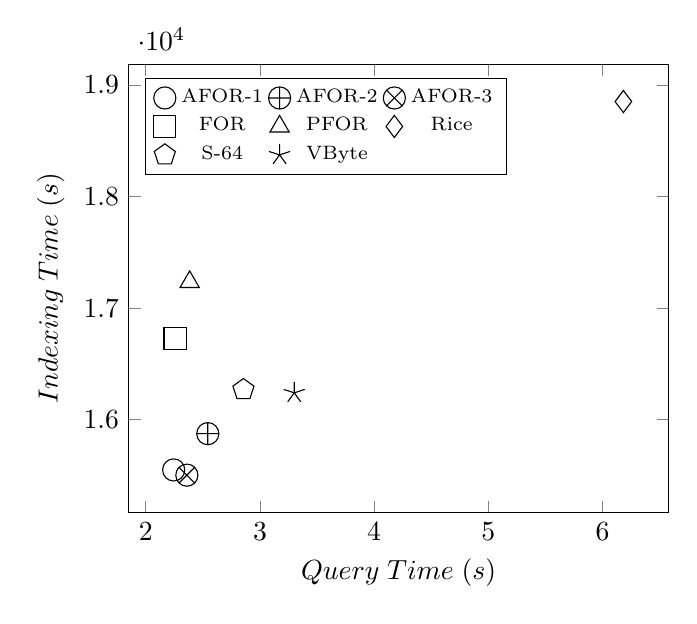
\begin{tikzpicture}
\begin{axis}[
  scatter/classes={
	a={mark=o},%
	b={mark=oplus},%
	c={mark=otimes},%
	d={mark=square},%
	e={mark=triangle},%
	f={mark=diamond},%
	g={mark=pentagon},%
	h={mark=star}
  },
  ylabel=$Indexing \; Time \; (s)$,
  xlabel=$Query \; Time \; (s)$,
  mark options={scale=2},
  legend columns=3,
  legend pos=north west,
  legend style={font=\scriptsize, anchor=north west, legend columns=3}
]

\addplot[only marks]
plot[scatter,mark=*,scatter src=explicit symbolic]
coordinates {
(2.2446, 15550) [a]
(2.5433, 15875) [b]
(2.3600, 15503) [c]
(2.2570, 16727) [d]
(2.3846, 17235) [e]
(6.1836, 18852) [f]
(2.8555, 16270) [g]
(3.3004, 16241) [h]
};
\legend{AFOR-1, AFOR-2, AFOR-3, FOR, PFOR, Rice, S-64, VByte}
\end{axis}
\end{tikzpicture}